\section{Inferential Statistics}
\subsection{Two-way analysis of variance(ANOVA)}
Our model is about using two-way ANOVA to determine the relationship between the dependent Processor Base Frequency with two independent which are number of Cores and Thermal Design Power(TDP). Because we want to check validity of this ANOVA model, we will have two assumption for this:\\
\\
\textbf{Normality}: Processor Base Frequency should be normal distribution for each combination of number of Cores and TDP.\\
\\
\textbf{Homogeneity}: Processor Base Frequency should be roughly across all combinations of number of Cores and TDP.
\subsubsection{Verify the assumption}
\textbf{Normality}: verify if the data is normal distribution\\
We use Shapiro-Wilk normality test to check if this model is normal distribution:\\
\\
\textbf{Null hypothesis $H_0$}: Processor Base Frequency should be approximately normally distributed for each combinations of number of Cores and TDP.\\
\\
\textbf{Alternative hypothesis $H_1$}: Processor Base Frequency should not be approximately normally distributed for each combinations of number of Cores and TDP.
\begin{figure}[H]
    \centering
    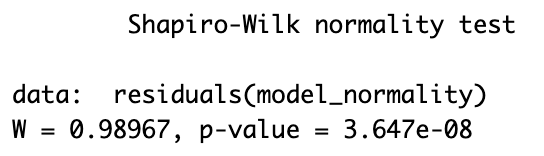
\includegraphics[width=0.8\textwidth]{graphics/shapiro.png}
    \caption{Shapiro-Wilk's test}
    \label{fig:shapiro}
\end{figure}
From the result, p-value is smaller than 0.05 so we reject $H_0$ and accept $H_1$. Therefore, Processor Base Frequency should not be approximately normally distributed for each combinations of number of Cores and TDP. So we need to plot out the model diagnose plot to check if it is normal distribution or not:
\begin{figure}[H]
    \centering
    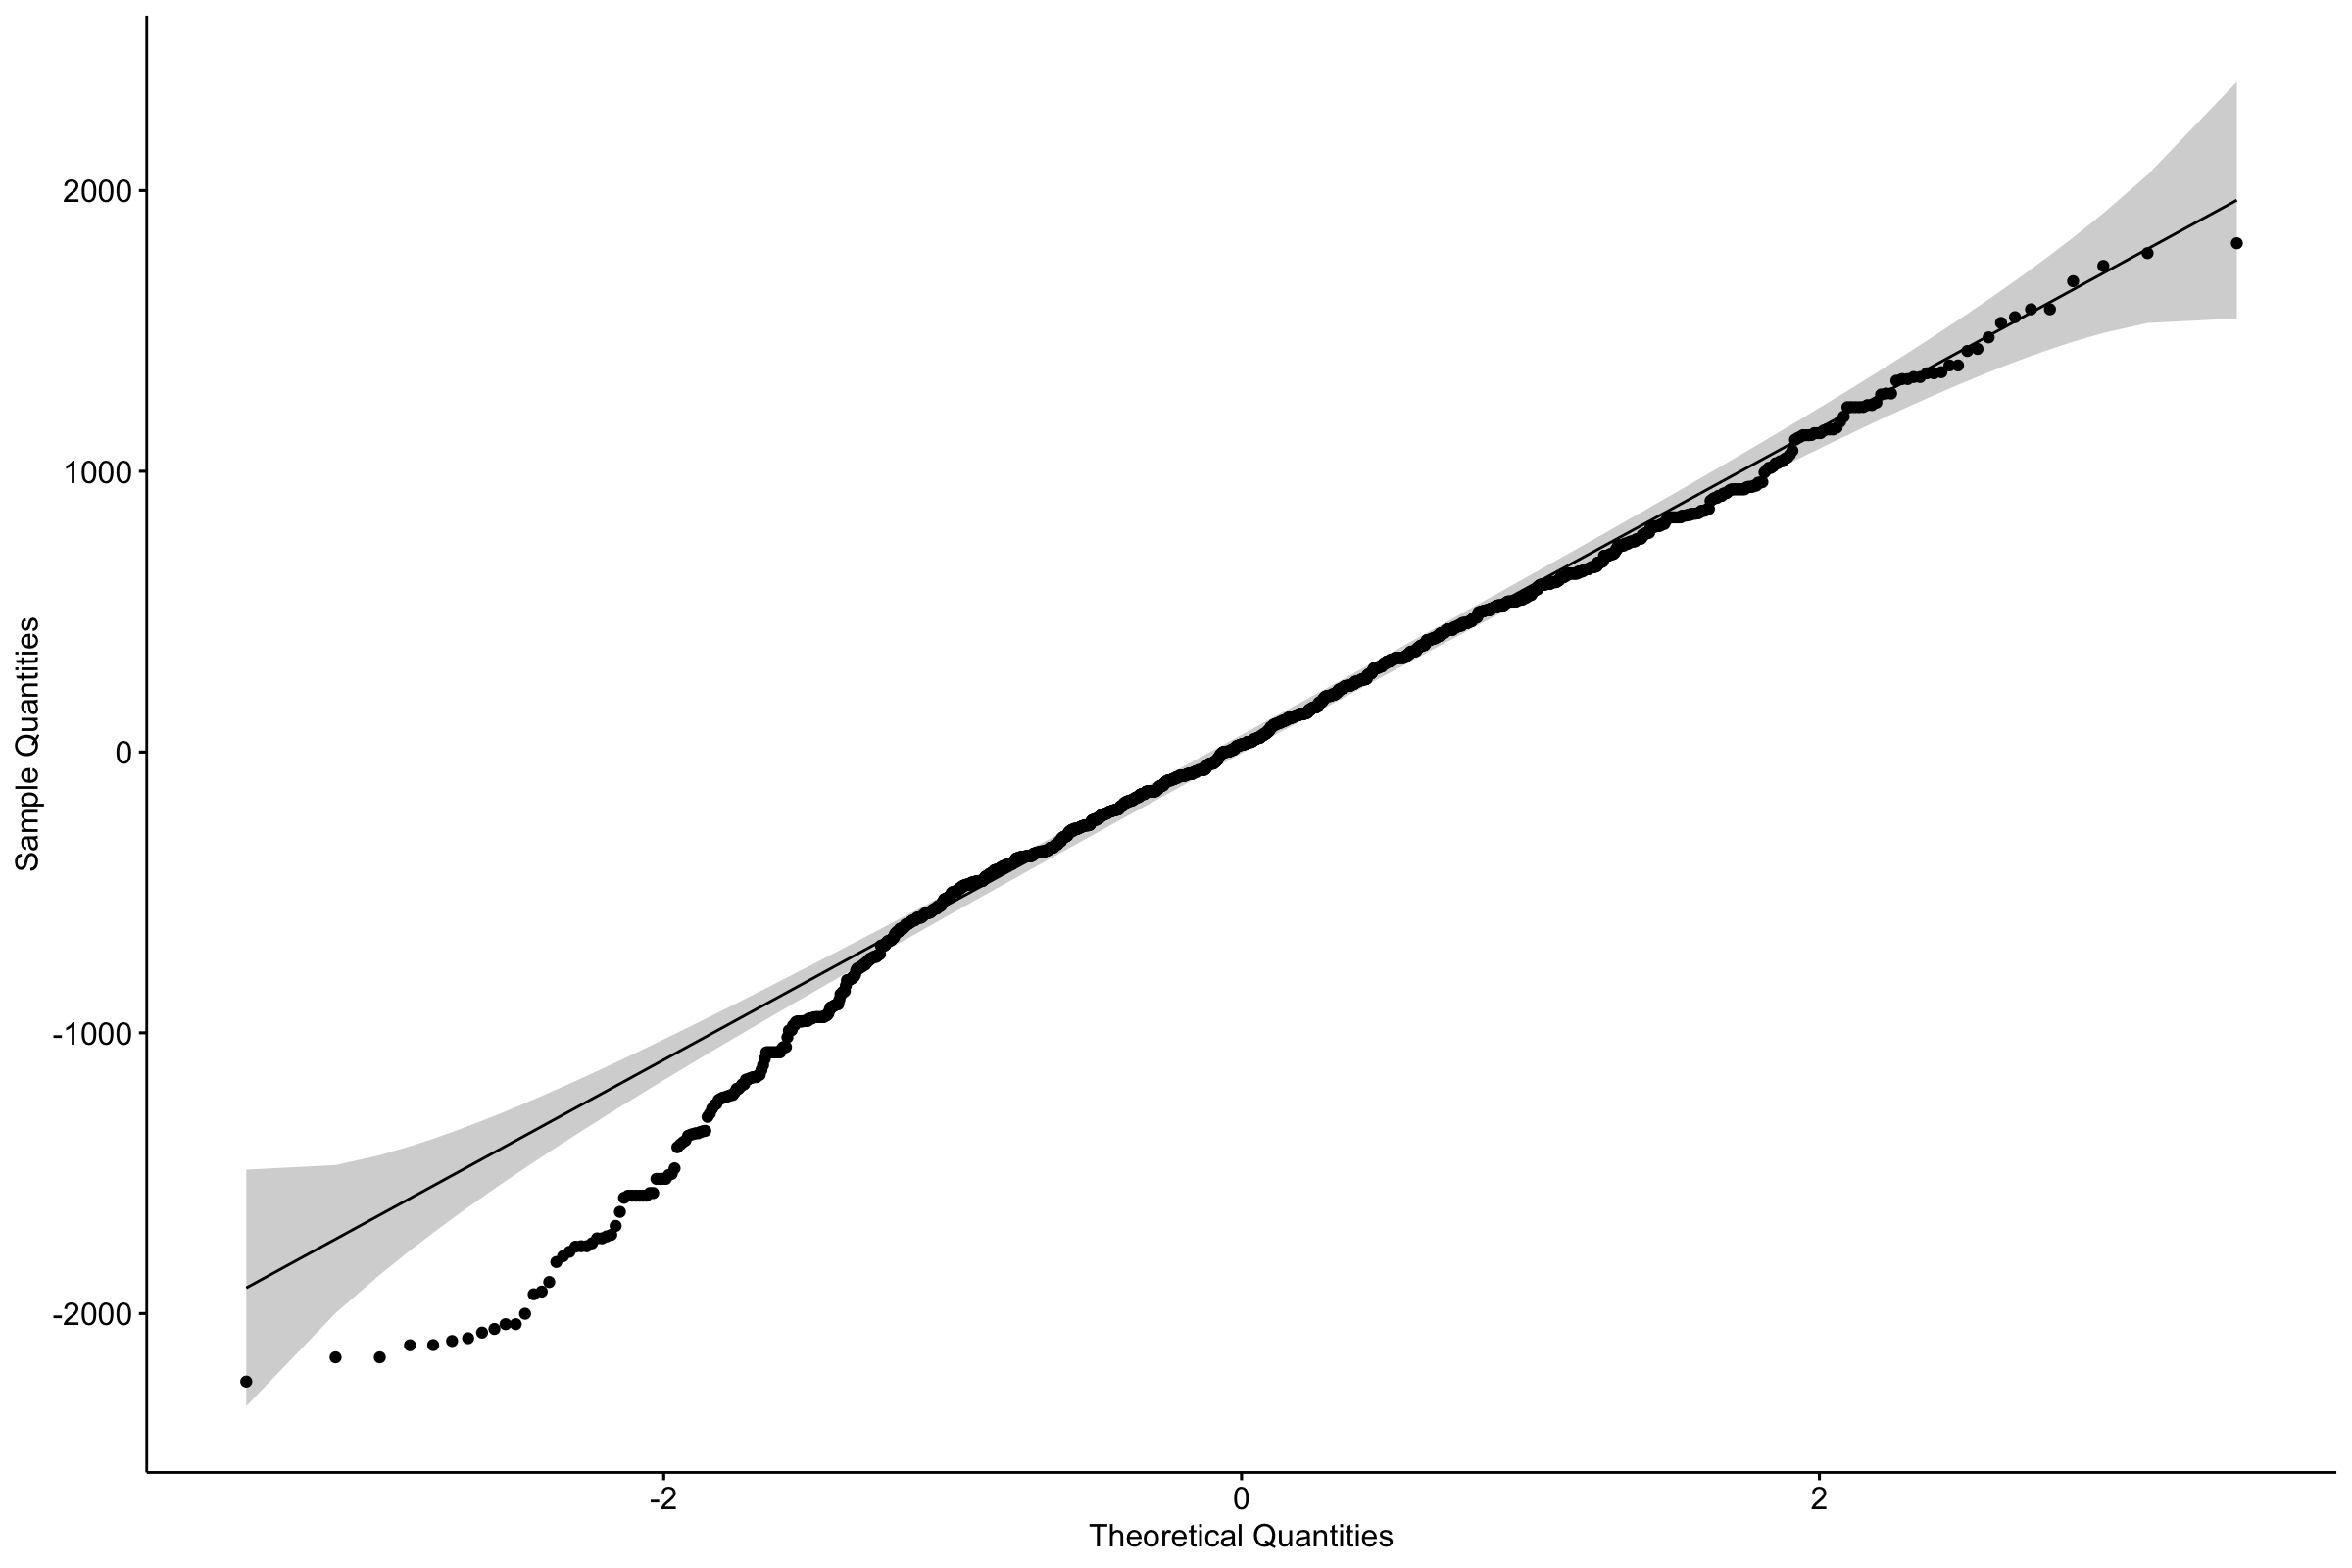
\includegraphics[width=1\textwidth]{graphics/check_normality.png}
    \caption{ggqqplot from ANOVA test}
    \label{fig:check_normality}
\end{figure}
We see that in ggqqplot, most of the points lie closely on the line. So we can assume that Processor Base Frequency is approximately normally distributed for each combinations of number of Cores and TDP.\\
\\
\textbf{Homogeneity}: verify the uniformity of the variance.\\
\\
We use Levene's test to check if this model is homogeneity:\\
\\
\textbf{Null hypothesis $H_0$}: Processor Base Frequency is homogeneity across groups of number of Cores and TDP.\\
\\
\textbf{Alternative hypothesis $H_1$}: Processor Base Frequency is not homogeneity across groups of number of Cores and TDP.
\begin{figure}[H]
    \centering
    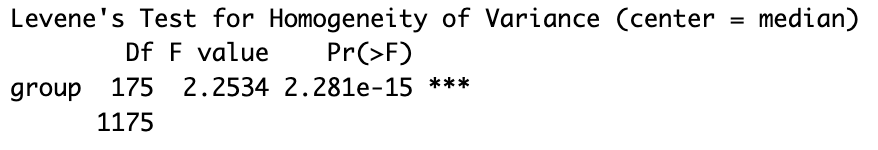
\includegraphics[width=1\textwidth]{graphics/check_homogeneity.png}
    \caption{Leneve's Test for Homogeneity of Variance}
    \label{fig:check_homogeneity}
\end{figure}
From the result, we see that p-value is smaller than 0.05 so we reject $H_0$ and accept $H_1$. Therefore, Processor Base Frequency is not homogeneity across groups of number of Cores and TDP. 
\subsubsection{Calculate ANOVA}
\textbf{Null hypothesis $H_0$}: Processor Base Frequency follows the same distribution across group defined by the independent variables number of Cores and TDP.\\
\\
\textbf{Alternative hypothesis $H_1$}: Processor Base Frequency follows different distribution across group defined by the independent variables number of Cores and TDP.
\begin{figure}[H]
    \centering
    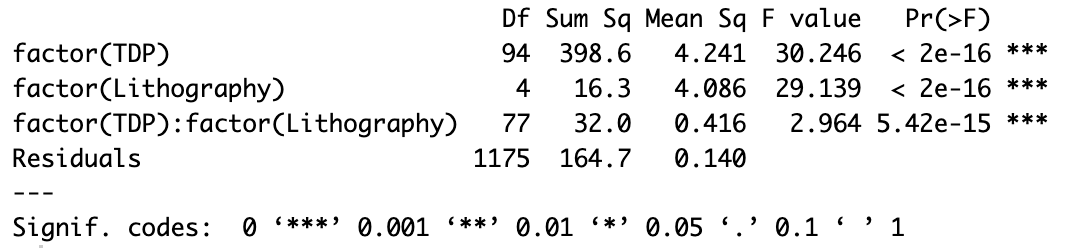
\includegraphics[width=1\textwidth]{graphics/anova_test.png}
    \caption{Calculate ANOVA}
    \label{fig:calculate_anova}
\end{figure}
From the result, we see that Pr(>F) value is smaller than 0.05 so we reject $H_0$ and accept $H_1$. Therefore, Processor Base Frequency follows different distribution across group defined by the independent variables number of Cores and TDP.

\subsection{Multiple Linear Regression to Predict CPU Clock Speed}
The main objective of this section is constructing a model that portrays the effect of other variables on the Processor Base Frequency. To achieve this we applied a Multi Regression model, in which the dependent variable is Processor Base Frequency, while the rest are independent. Our model comes in this form:

%ai thêm giùm cái pt regression nha :3

We start with our first model, also known as the base model, where it will be built with all the independent variables available.

%ảnh model 2

In this model, our independent variables consist of: 



\subsection{Result}

\newpage
